The evaluation of a drone programming system is crucial to assess its effectiveness, performance, and suitability for specific applications. 
This chapter aims to provide a comprehensive evaluation of EasyFly. 
The baseline used to compare our programming environment is the basic Crazyflie python library (cflib) 

We divided the evaluation process into two main topics: we will give a qualitative analysis of EasyFly and an understanding of the strengths and leaks of our programming system.
For this analysis, we participated in the challenges organized for the Digital Futures Drone Arena project~\cite{dronearena}.
During this challenge, groups of students and enthusiasts were asked to complete an obstacle run using Crazyflie 2.1 nano drones.

Then, we will move to performance analysis of EasyFly in a real example implementation, comparing it with a similar implementation written using only the core cflib.
This evaluation aims to assess the ease of implementing a drone application with EasyFly and the consequent reduction in complexity in the scripts. 
On the other hand, we will demonstrate that the performance of an application developed with EasyFly is almost the same as the implementation using the core cflib offered by Crazyflie.
In this second part, we will describe the EasyFly simulation environment that allowed us to conduct a precise performance analysis.

\section{Qualitative Analysis}\label{sec:qualitative_analysis}
In the HDI domain, the research's core part, especially from the computer science perspective,
is the experimental phase. During this phase, researchers put their ideas and prototypes to test
and assess the practicality of innovative interaction models.

For a programming environment like EasyFly, testing and evaluating in a real research scenario in HDI is essential. 
The testing in real scenarios can help detect possible weaknesses in the programming environment, allowing for fine-tuning the model.

To best evaluate our EasyFly programming environment, we had the possibility to participate in the Digital Futures Drone Arena project~\cite{dronearena}.

The Drone Arena project planned two challenges where groups of students and enthusiasts with different backgrounds were asked to complete a specific task using drones.
These challenges aim to allow researchers to collect data and perform studies about human-drone interactions.

The EasyFly programming environment was part of the inaugural challenge in Sweden in June 2022~\cite{dronearenaChallenge}. 
In this challenge, five groups of students and enthusiasts with knowledge of computer science were asked to program Crazyflie 2.1 nano drones to complete an obstacle course.
There were two main alternatives to write the scripts: the standard cflib or the EasyFly programming environment. 

The challenge was distributed over three days; the first two days were dedicated to development and testing, and the last day was dedicated to the final challenge, where the groups competed with each other with what they had produced in the days before.
On the first day, we gave the groups a brief presentation on the basic knowledge of the Crazyflie 2.1 platform. 
We also described the main components and working principles of the EasyFly programming environment.
Then, we provided the groups with a Python project, where inside was the original cflib, our EasyFly programming environment, and a folder of examples for both.
From then on, the groups were free to develop and test the code with real Crazyflie 2.1 in a sample stage, with minimum support from the research team.

This particular setting of the challenge allowed us to see and measure the impact of using EasyFly on a group with minimum knowledge of the Crazyflie platform. 
On the final day of the challenge, 2 out of 5 teams decided to participate in the final using our EasyFly programming environment. 

The approach for all the groups was to use a Multiranger deck and perform a hand-driven flight through the obstacle course.
The main differences were how the groups implemented the mechanism that allowed them to push or pull the drone using their hands.

By analyzing the code that all the groups produced, we noticed two main aspects of the usage of the EasyFly programming environment:
The groups that started using EasyFly from the beginning developed more complex solutions.
The code of the groups that used the programming environment looked clean and simple, even if the solution they implemented was more complex.

Although we expected more adhesion on EasyFly, we noticed that almost all the groups had a look at the code of the programming environment, in particular inside the utility functions of the ECF modules. 
In their final code, almost every group used the utility functions of the Multiranger ECF Module, either directly or indirectly.

In conclusion, the challenge of the Drone Arena project allowed us to understand that the entire EasyFly programming environment, particularly the Coordination Manager, can seem too complicated at first glance and was a little more complex than we thought.
The groups that decided not to use the programming environment decided on purpose to develop a more simple and sometimes effective solution.


\section{Performance Analysis}\label{sec:performance_analysis}

EasyFly is a programming environment that aims to ease the development of drone applications, reaching the same solution with less effort, both in terms of time to write the solution and expertise required to implement the solution.
Even if simplicity remains the first objective, performance plays an important role in the EasyFly programming environment.

If the programming environment is easy to use but, in the end, results in inefficiency in terms of performance, it automatically becomes useless.
To assess the performance of EasyFly, we compared it with the standard implementation of Crazyflie cflib across two real example applications.
In this analysis, we will demonstrate that the expected loss in performance with respect to the basic cflib implementation is shallow compared to the reduction of program complexity.

\subsection{EasyFly Simulation Environment}\label{subsec:simulation_environment}
Measuring performance in drone applications is a very hard task. 
Usually, the performance of the applications can vary highly across different runs.
The only possible strategy to measure performance is to execute and measure the same scenario multiple times and then average the results.

To simplify the evaluation process and collect more precise data, we developed a simulation environment for EasyFly.
Given that the scripts written using our EasyFly programming environment are meant to run on the ground station, 
in our simulation environment, these scripts connect to a virtual Crazyflie 2.1 using a local UDP communication channel.

Figure~\ref{fig:simulation_environment} represents the basic infrastructure of the simulation environment: 
The virtual Crazyflie is hosted on a Python script that uses a bidirectional UDP channel to handle the communications to and from the EasyFly script.

\sidecaptionvpos{figure}{c}
\begin{SCfigure}[\sidecaptionrelwidth][h]
    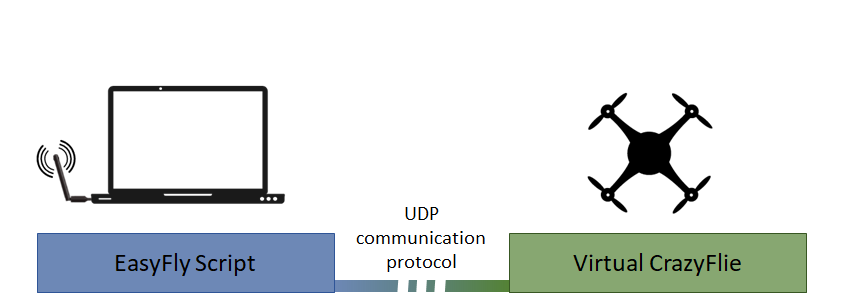
\includegraphics[width=0.5\textwidth]{evaluation/simulation_environment}
    \caption{Structure of EasyFly simulation environment}\label{fig:simulation_environment}
\end{SCfigure}

Upon receiving the commands, the virtual Crazyflie updates its internal state and sends back data, emulating a real Crazyflie 2.1.
In the current implementation of the EasyFly simulation environment, the virtual Craziflie emulates the control-related commands, logging, and parameter features.

\subsection{Tools and Metrics for Measuring Performances}\label{subsec:performance_metrics}

To measure the performance of our programming environment, we targeted two main categories of performance metrics: execution performance and complexity.
The first category of metrics, the execution performances, is a set of metrics that measures the resource consumption of the scripts.
The category is composed of the following metrics:
\begin{itemize}
    \item Memory (RAM) consumption
    \item Average CPU consumption 
    \item Max CPU consumption
    \item Network load (?) 
\end{itemize}

To measure the memory consumption, we used \textit{memory-profiler}~\cite{memoryProfiler}, a Python library for collecting RAM usage during the execution of a Python script.
We used the \textit{Performance Monitor} tool for Windows for the CPU metrics. 
Finally, the simulation environment automatically computes the network load by summing all the CRTP received and sent.

The second category, complexity, is a set of metrics that tries to evaluate the complexity of a program.
The category is composed of the following metrics:
\begin{itemize}
    \item Cyclomatic Complexity -- the number of linearly independent paths through the code
    \item LOC -- total number of lines of code
    \item Halstead Metrics 
    \item Maintainability index -- measures the source code's maintainability (easy to support and change).
\end{itemize}

To collect all these measurements, we used \textit{radon}~\cite{radon}, a Python library that computes all such metrics using static analysis on the source code of the scripts.